\documentclass[%
 aip,jap,
% jmp,
% bmf,
% sd,
% rsi,
 amsmath,amssymb,
preprint,%
% reprint,%
% floatfix,
%author-year,%
%author-numerical,%
% Conference Proceedings
]{revtex4-1}

\usepackage{graphicx}% Include figure files
\usepackage{dcolumn}% Align table columns on decimal point
\usepackage{bm}% bold math
%\usepackage[mathlines]{lineno}% Enable numbering of text and display math
%\linenumbers\relax % Commence numbering lines

\usepackage[utf8]{inputenc}
\usepackage[T1]{fontenc}
\usepackage{mathptmx}
\usepackage{etoolbox}

%% Apr 2021: AIP requests that the corresponding
%% email to be moved after the affiliations
\makeatletter
\def\@email#1#2{%
 \endgroup
 \patchcmd{\titleblock@produce}
  {\frontmatter@RRAPformat}
  {\frontmatter@RRAPformat{\produce@RRAP{*#1\href{mailto:#2}{#2}}}\frontmatter@RRAPformat}
  {}{}
}%
\makeatother

\begin{document}

%\title{Supplementary material}
%%\section*{Supplementary material}
%
%\maketitle

\section*{Supplementary material}

\begin{figure}[!b]
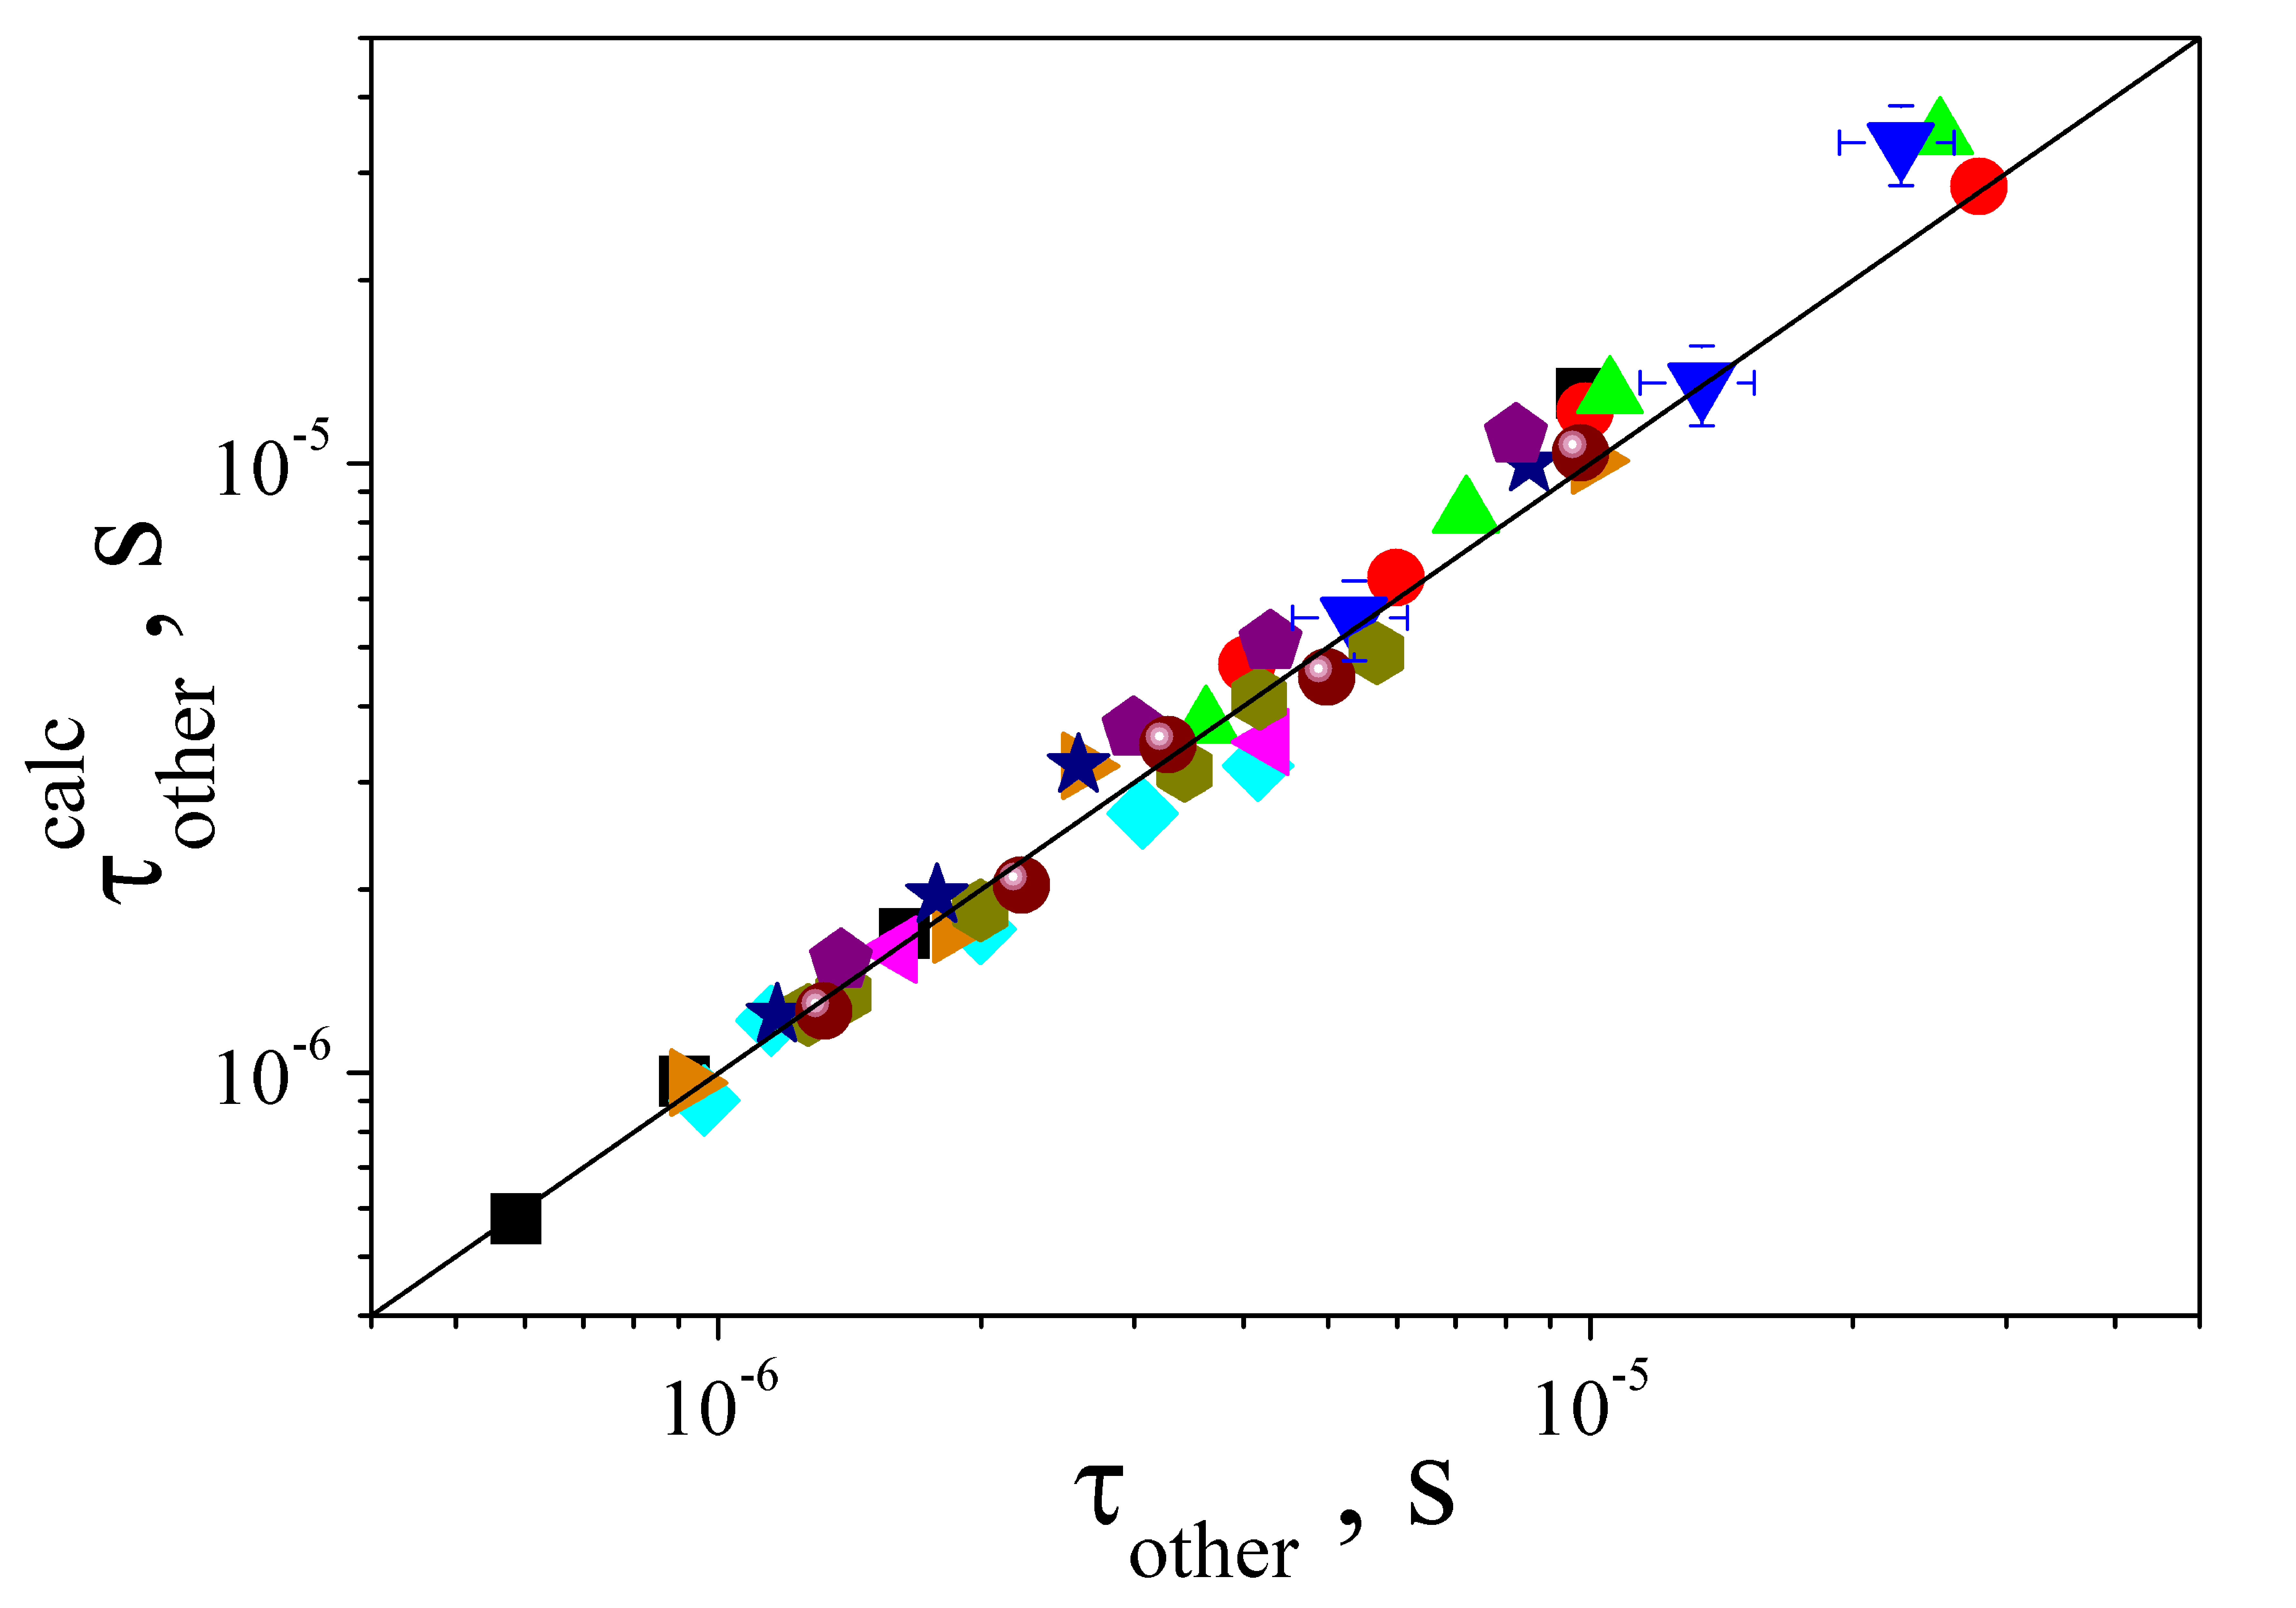
\includegraphics[width=0.5\textwidth]{FigS1}% Here is how to import EPS art
\caption{\label{Fig:TauOther}
$\tau_\mathrm{other}$ is plotted against those calculated from
$N_\mathrm{Fe,0}$ and $N_\mathrm{Fe,fit}$ values (see paper text).
Different points mark different samples and illumination conditions.
The black solid line is the identify line servings as the references.
}
\end{figure}


\end{document}

